\documentclass[a4paper,10pt,twoside,final,spanish]{article}

% Preámbulo - Parte A

\usepackage[utf8]{inputenc} % Soporte para los acentos
\usepackage[T1]{fontenc}

\usepackage[spanish]{babel} % Capítulos, seciones, etc. en español

\usepackage[margin=1.5cm]{geometry} % Diseño del documento

\usepackage{enumerate} % Cambiar etiquetas de numeración
\usepackage[shortlabels]{enumitem} % Manejo adicional de etiquetas de numeración

\usepackage{graphicx} % Manejo de gráficos y figuras

\usepackage{xcolor} % Usar colores
\usepackage{pstricks}

\usepackage{makeidx} % Índice alfabético

\usepackage{textcomp}
\usepackage{amsmath}
\usepackage{amsfonts}
\usepackage{amssymb}
\usepackage{hyperref}

%---
\usepackage{geometry} %Algo de las líneas del pie y encabezados
\geometry{text={7in,9.5in},headheight=15pt}
%\textwidth = 7 in
%\textheight = 9.5 in
%\oddsidemargin = -0.25 in
%\evensidemargin = 0.0 in
%\topmargin = -0.25 in
%\headheight = 0.0 in
%\headsep = 0.0 in
\setlength{\parskip}{0.1in}
\setlength{\parindent}{0.0in}
%---
\usepackage{fancyhdr} %Para usar encabezados y pies personalizados
	\pagestyle{fancy}
	\fancyhf{}
	\fancyhead[LE,RO]{Tecnologías para la Web Semántica} 
	\fancyhead[RE,LO]{Methontology}
	\fancyfoot[RE,LO]{Darién Julián Ramírez}
	\fancyfoot[LE,RO]{\thepage}
	\renewcommand{\footrulewidth}{1pt}
%---
\usepackage{listings} %Para escribir códigos
\lstset{language=XML,
	basicstyle=\footnotesize,
	numbers=left,
 	stepnumber=1,
	numbersep=8pt,
	showspaces=false,               % show spaces adding particular underscores
  	showstringspaces=false,         % underline spaces within strings
  	frame=lines,                   % adds a frame around the code
	tabsize=4,                      
  	captionpos=b,                   % sets the caption-position to bottom
  	breaklines=true,                % sets automatic line breaking
}
%---

% Preámbulo - Parte B

\title{\Huge Tecnologías para la Web Semántica\\
			 Trabajo Práctico Nº7\\
			 Documento de Especificación}
\author{Darién Julián Ramírez}
\date{}

% Cuerpo del documento

\begin{document}

\maketitle % Mostrar título

\section*{Ejercicio 1}

Elabore el documento de especificación de una ontología sobre una plataforma de series online. Esta plataforma permite elegir contenidos en un catálogo de series. El contenido seleccionado puede ser visualizado en Smart TV, consolas de juegos, PC, Mac, dispositivos móviles o tablets conectados a internet. La propuesta no implica descarga de contenidos sino que estos se visualizan en tiempo real (leer \textit{Todo lo que Netflix sabe de vos}).

\textit{Aclaración:} Siga las actividades propuestas en la metodología Methontology.\\

\framebox{
\begin{minipage}{0.5\textwidth}
\textbf{Documento de especificación de ontologías} \\

\textbf{Contenido:}
\begin{itemize}
\item \textbf{Propósito.}
\item \textbf{Escenarios de uso.}
\item \textbf{Posibles usuarios finales.}
\item \textbf{Preguntas de competencia.}
\end{itemize}
\end{minipage}
}

\dotfill

\begin{quote}

\begin{center}
\textbf{DERO. Documento de especificación de requerimientos sobre una ontología de la plataforma de series online Netflix}
\end{center}

\begin{itemize}
\item \textbf{Propósito:}

Ofrecer a los clientes contenidos online de series y películas que podrá ser visualizado desde diferentes dispositivos sin permitir la descarga de contenido.
Conectar a los clientes con grandes historias. Ofrecer a los clientes sugerencias personalizadas para encontrar mejores contenidos más fácil y rápido.

\item \textbf{Escenarios de uso:}

	\begin{itemize}
	\item Suscripción a Netflix.
	\item Selección de contenido.
	\item Obtención de información sobre los clientes como ayuda para la toma de 			decisiones. 
	\end{itemize}

\item \textbf{Posibles usuarios finales:}

Toda aquella persona o grupo suscrita/o al servicio de televisión online Netflix.

\item \textbf{Preguntas de competencia:}

	\begin{itemize}
	\item ¿Qué tipo de contenido prefiere el cliente?
	\item ¿Cómo usar los metadatos para determinar las preferencias del cliente?
	\item ¿A qué hora se conecta un cliente?
	\item ¿Qué contenido mira un cliente?
	\item ¿Qué capítulos en específico mira el cliente en una sesión?
	\item ¿Desde qué dispositivo utiliza Netflix un cliente?
	\item ¿Cuál es la marca y modelo del dispositivo?
	\item ¿Qué navegador de internet utilizó el cliente para conectarse?
	\item ¿Cuál es la dirección de IP del cliente?
	\item ¿Ha perdido el cliente el interés en algún contenido?
	\item ¿Cuántos minutos de un contenido ha visto el cliente?
	\item ¿Cuántas pausas ha realizado el cliente durante la reproducción del 				contenido?
	\item ¿Cuánto tiempo han durado esas pausas?
	\item ¿Está el cliente \textit{enganchado} a determinado contenido?
	\item ¿Cuál es el contenido al cual el cliente no está \textit{enganchado}?
	\item ¿Qué palabras clave ha utilizado el cliente para la búsqueda de contenido?
	\item ¿El cliente, ha hecho clic?
	\item ¿Cuál es el historial de búsquedas del cliente?
	\item ¿Qué puntuación ha dado el cliente a un contenido?
	\item ¿Cuál es el medio de pago del cliente?
	\item ¿Cuál es el total de horas de contenido vistas por el cliente?
	\item ¿Cuál es el número de programas y series que ha visto el cliente?
	\item ¿Cuánto ha pagado el cliente hasta el momento?
	\item ¿Cuál es el \textit{episodio gancho} de un cliente para un determinado 			contenido?
	\item ¿Cuál es la información personal del cliente?
	\end{itemize}

\end{itemize}

\end{quote}

\section*{Ejercicio 2}

Elabore el modelo según la especificación de requerimientos realizada en el punto 1.

\dotfill

\begin{center}
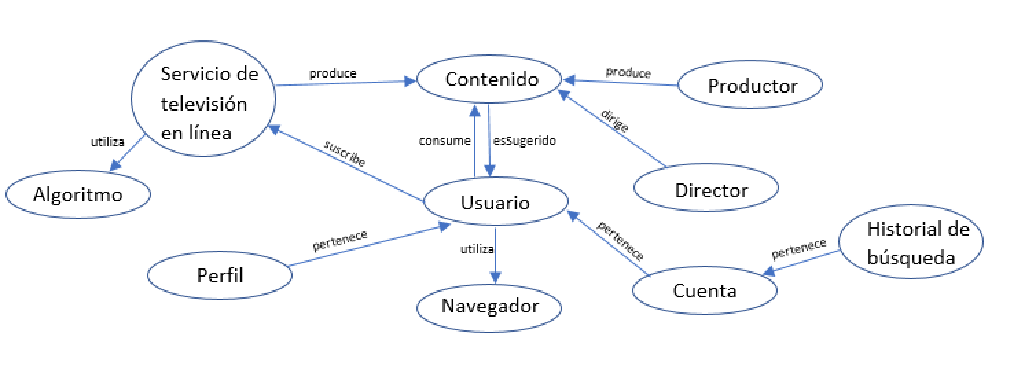
\includegraphics[width=\linewidth]{modelo2}
\end{center}

\begin{itemize}
\item Una película \textit{es un} contenido.
\item Una serie \textit{es un} contenido.
\end{itemize}

\begin{center}
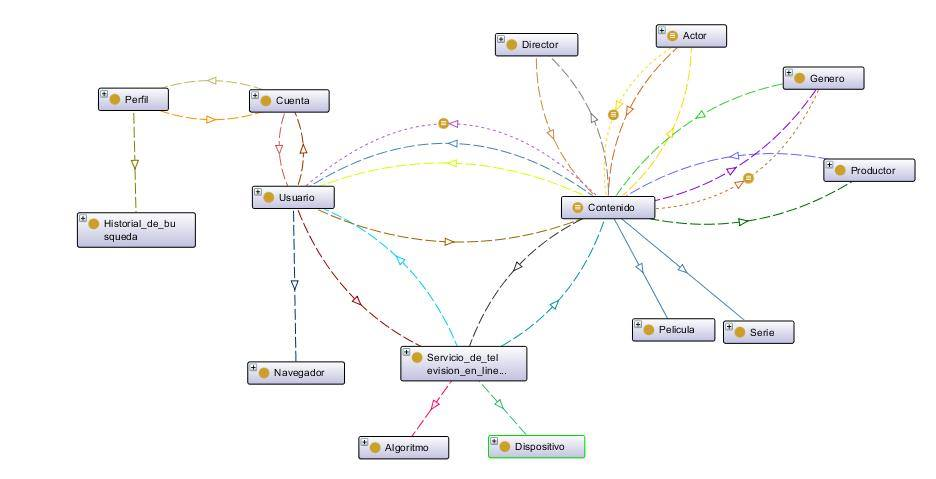
\includegraphics[width=\linewidth]{modelo3}
\end{center}

\section*{Todo lo que Netflix sabe de vos (y para qué quiere saber tanto)}

Los hábitos de sus usuarios son una fuente de información fundamental para que la compañía decida qué contenido ofrecer.

\begin{figure}[!htbp]
\centerline{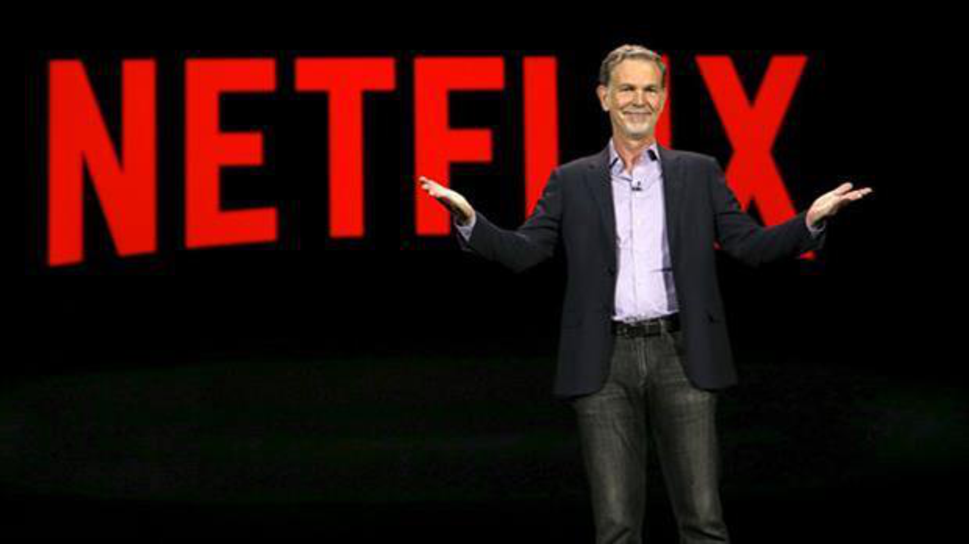
\includegraphics{img1}}
\caption{Reed Hastings, creador de Netflix.}
\label{fig:img1}
\end{figure}
 
Mientras vos mirás Netflix, Netflix te mira a vos. El servicio de televisión en 
línea es cada vez más popular. En 2016 batió su récord de suscriptores 
internacionales y ya está disponible en 190 países, según explica en su sitio 
web. En total, cuenta con más de 100 millones de clientes en todo el 
mundo.

Y una de las claves de su éxito es, sin duda, la profundidad con la que 
conoce a su público: Netflix estudia con detalle tus hábitos de consumo 
para conocerte mejor y para sacarte el mejor partido como usuario.
 
Ya lo dijo hace tiempo el gurú mundial de marketing Philip Kotler: \textit{Lo más importante es predecir hacia dónde van los clientes y pararse en frente de ellos}. Y eso es, precisamente, lo que hace Netflix cada vez que te conectás a su servicio.
 
La clave: los metadatos, los grupos de datos que definen tu perfil gracias a la información que le das cada vez que mirás uno de sus videos (e incluso antes de hacerlo), y que de ser interceptados pueden dar muchísima información sobre tus gustos.

Netflix observa a qué hora te conectaste para ver el último capítulo de tu serie favorita (y el primero), desde dónde lo hiciste exactamente y cuándo perdiste el interés. Analiza también cuántos minutos de la serie viste, cuántas pausas hiciste y cuánto duró cada una de ellas. Sabe si estás \textit{enganchado} a una serie, película o documental, o si no logró atraparte del todo.

\textbf{Lo que ves... y lo que querés ver}
 
Netflix conoce los perfiles de sus clientes y reconoce los dispositivos desde el que te conectás cuando accedés a su web: qué modelo y marca de televisor, smartphone o tableta usás en cada ocasión y cuál es tu navegador de internet y la dirección IP de tu terminal. También sabe qué palabras escribís en el buscador para acceder a las series y películas que ofrece, y cuándo hacés clic (y cuándo no).
 
\begin{figure}[!htbp]
\centerline{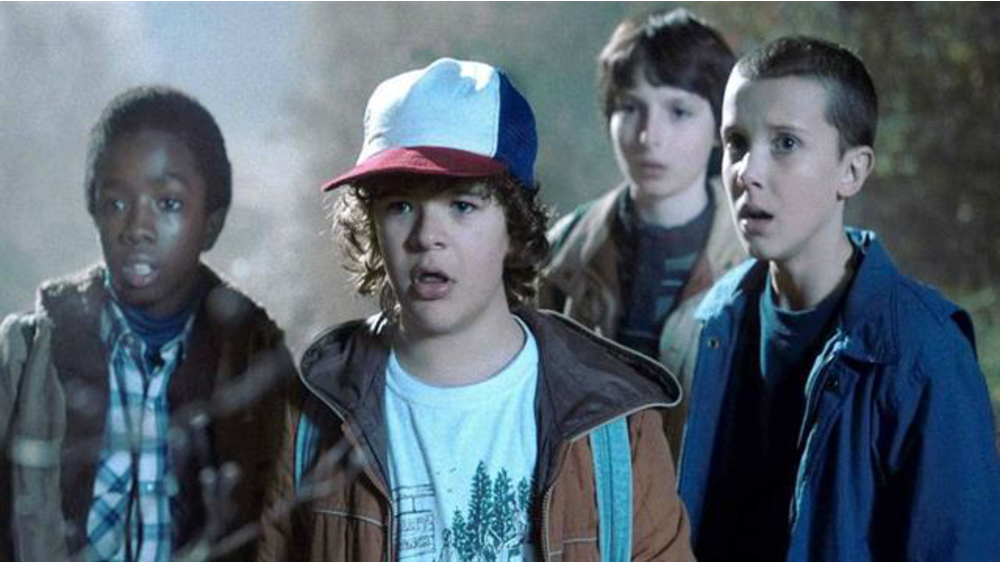
\includegraphics{img2}}
\caption{Stranger Things, uno de los éxitos de Netflix. Foto: Archivo}
\label{fig:img2}
\end{figure}
 
Sabe también cuál es tu historial de búsquedas, qué productos te gustan más, cómo los puntuás y, por supuesto, cómo pagás sus servicios. Tiene un recuento del número de horas de contenidos audiovisuales que has visto desde que tenés la cuenta, cuántos programas y series has consumido y cuánto has pagado por ellos.

En 2015, la compañía tecnológica lanzó una estadística muy interesante en la que reveló que conoce el momento exacto en el que sus usuarios se \textit{enganchan} a sus series. Es lo que llama el \textit{episodio gancho}.

Apenas conoce los datos personales de sus clientes, más allá de su nombre, correo electrónico y datos de facturación, pero gracias a todos los metadatos que tiene sobre ellos es capaz de hacer un perfil comercial que les define y de incluirles en categorías según sus hábitos e intereses. Y no lo oculta.

\textbf{El poder de los algoritmos}
 
En el blog empresarial de Netflix hay una larga lista de comunicados de prensa en los que da a conocer datos que analizó para mostrar el comportamiento de sus usuarios. \textit{El 58\% de los mexicanos se adelanta a su pareja en los episodios de las series}, proclama en uno de ellos.

Y justifica de esta manera su afán por saberlo todo sobre vos: \textit{En Netflix nuestra meta es conectarte con grandes historias. Cada uno de nuestros miembros tiene gustos únicos y trabajamos constantemente para mejorar las sugerencias personalizadas que permiten encontrar los mejores contenidos más fácil y rápido.}
 
\begin{figure}[!htbp]
\centerline{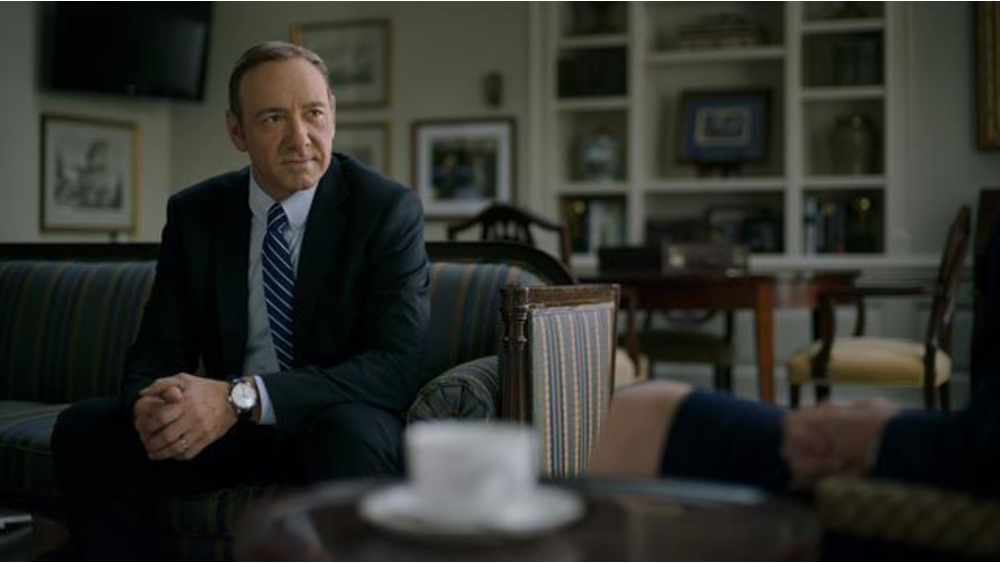
\includegraphics{img3}}
\caption{House of Cards, la serie que más hizo para impulsar el crecimiento de Netflix. Foto: Archivo}
\label{fig:img3}
\end{figure}

La compañía se define como \textit{la principal red de televisión por internet del mundo}. Y sus más de 125 millones de horas de programas de televisión y películas por día le avalan.

\textit{Todos los datos son alimentados por distintos algoritmos, cada uno de ellos optimizado para diferentes propósitos}, le contó a la revista tecnológica Wired Xavier Amatriain en 2013, cuando era director de ingeniería de la compañía.

Según Amatriain, los algoritmos -programas de computadoras que resuelven problemas- dividen a cada usuario según sus gustos y usan ese comportamiento para establecer cuáles son sus preferencias. \textit{Sabemos lo que has reproducido, lo que has buscado o lo que has calificado}, dijo el exdirectivo de Netflix, quien ahora trabaja para el sitio de preguntas y respuestas Quora.

Gracias a esos algoritmos, Netflix decidió cambiar sus patrones en 2013 y apostar por su propio material, ofreciendo las 13 primeras entregas seguidas de la serie House of Cards, que pagó por adelantado, en lugar de probar primero con un episodio piloto.

\begin{figure}[!htbp]
\centerline{
\includegraphics{img4}}
\caption{Sense8, otro de los contenidos exclusivos. Foto: Netflix}
\label{fig:img4}
\end{figure}
 
Los datos sobre el contenido más visto y amado por sus clientes revelaron tres ingredientes claves: el actor Kevin Spacey, el director David Fincher y los dramas políticos producidos por la BBC. Así que la empresa encargó una nueva versión de la serie, la cual llegó a ganar el prestigioso premio Emmy. Y demostró así que los algoritmos tenían razón (y sabían mucho sobre sus usuarios).

Los datos no sólo le sirven a Netflix para saber lo que funciona, sino también lo que puede funcionar en el futuro. Y es que Netflix, más que mirarte, te examina. Y cada dato que obtiene lo guarda cuidadosamente dentro de su almacén digital. Si querés saber lo que sabe sobre vos, tan sólo tenés que preguntárselo. Las leyes de protección de datos personales le obligan a contártelo, si se lo solicitás. Pero saberlo no evitará que deje de hacerlo: Netflix te seguirá observando, lo quieras o no.

\begin{thebibliography}{99}
\bibitem{SWP}
Grigoris Antoniou and Frank van Harmelen,
\emph{A Semantic Web Primer}, segunda edición.
The MIT Press, Cambridge, Massachusetts; London, England,
2008.
\end{thebibliography}

\end{document}